% Modelo para apresentação Beamer IFSC
\documentclass{beamer}

\usepackage[utf8]{inputenc}
\usepackage[T1]{fontenc}
\usepackage[english,brazil]{babel}
\usepackage{amsmath, amssymb, graphicx, caption}
\usepackage{beamerthemeIFSC}

\title{EDB18802 - Eletrônica Digital II:}
\subtitle{\LARGE Registradores}
\author{João Cláudio Elsen Barcellos}
\date{\scriptsize \the\day~de \ifcase\month\or Janeiro\or Fevereiro\or Março\or Abril\or Maio\or Junho\or Julho\or Agosto\or Setembro\or Outubro\or Novembro\or Dezembro\fi~de \the\year}
\institute{Engenheiro Eletricista \\ Universidade Federal de Santa Catarina \\ \url{joaoclaudiobarcellos@gmail.com}}

\begin{document}

\frame{\titlepage}

\begin{frame}{Plano de Aula}
\tableofcontents
\end{frame}

\section{Introdução}



\begin{frame}{O que são Registradores?}
\begin{itemize}
    \item Circuito sequencial formado por flip-flops.
    \item Armazenam e deslocam dados binários.
    \item Cada flip-flop armazena um bit.
    \item Usados para transferência, armazenamento e conversão de dados.
\end{itemize}
\end{frame}



\begin{frame}{O que são Registradores?}
\begin{itemize}
\item O uso mais comum de flip-flops é no armazenamento de dados binários. 

\item Esses dados são geralmente armazenados em grupos de flip-flops denominados registradores. 

\item Basicamente, um registrador consiste em um grupo de FF tipo D que atuam no armazenamento de dados binários, pois um FF tem a capacidade de armazenar somente um bit, e de realizar a transferência dele. 

\end{itemize}
\end{frame}


\begin{frame}{O que são Registradores?}
\begin{itemize}
    \item O dado binário dentro de um registrador pode ser movido de um flip-flop para outro. Os registradores que permitem tal transferência são denominados de registradores de deslocamento (shift-register). 

    \item Há 4 modos de operação básicos de um registrador:

• Registrador série/série\\
• Registrador série/paralelo\\
• Registrador paralelo/paralelo\\
• Registrador paralelo/série\\

\end{itemize}
\end{frame}



\section{Tipos de Registradores}

\begin{frame}{Série-Série}
\begin{itemize}
    \item Entrada e saída serial (bit a bit).
    \item Requer vários pulsos de clock.
\end{itemize}
\end{frame}

\begin{frame}{Exemplo - Série-Série}
\centering
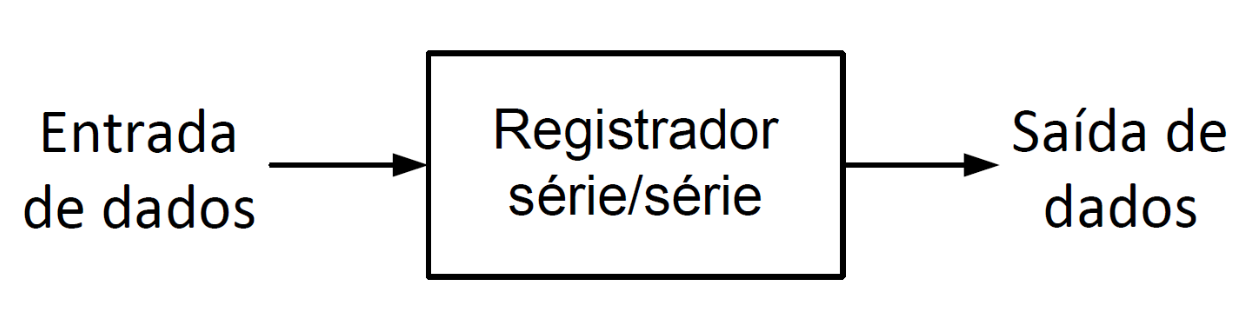
\includegraphics[width=0.65\textwidth]{figures/serie_serie.png}
\end{frame}

\begin{frame}{Série-Paralelo}
\begin{itemize}
    \item Entrada serial (bit a bit), saída paralela (todos os bits ao mesmo tempo).
    \item Usado para converter dados seriais em paralelos.
\end{itemize}
\end{frame}

\begin{frame}{Exemplo - Série-Paralelo}
\centering
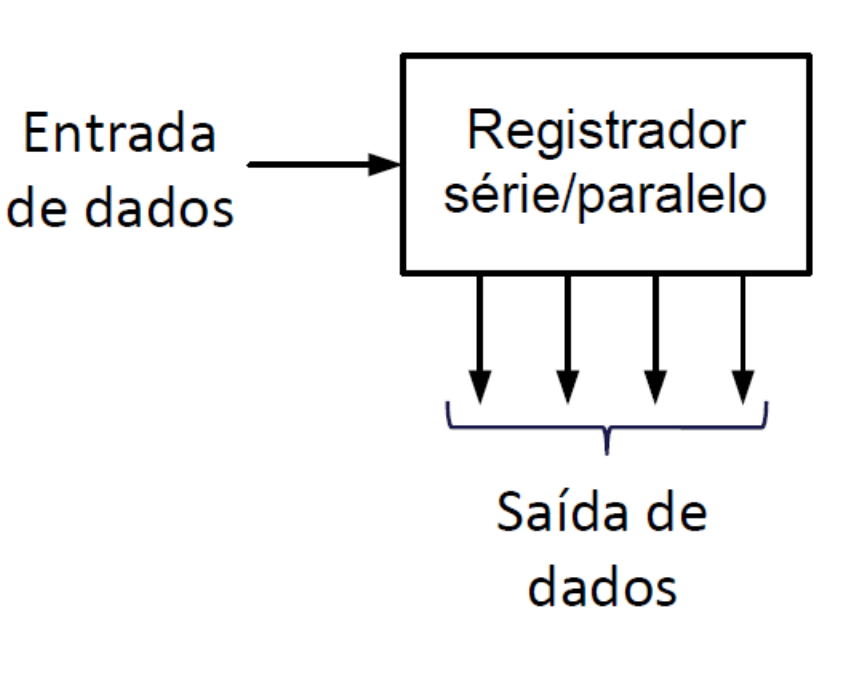
\includegraphics[width=0.65\textwidth]{figures/serie_paralelo.png}
\end{frame}

\begin{frame}{Paralelo-Série}
\begin{itemize}
    \item Entrada paralela, saída serial.
    \item Usado em comunicação com dispositivos seriais.
\end{itemize}
\end{frame}

\begin{frame}{Exemplo - Paralelo-Série}
\centering
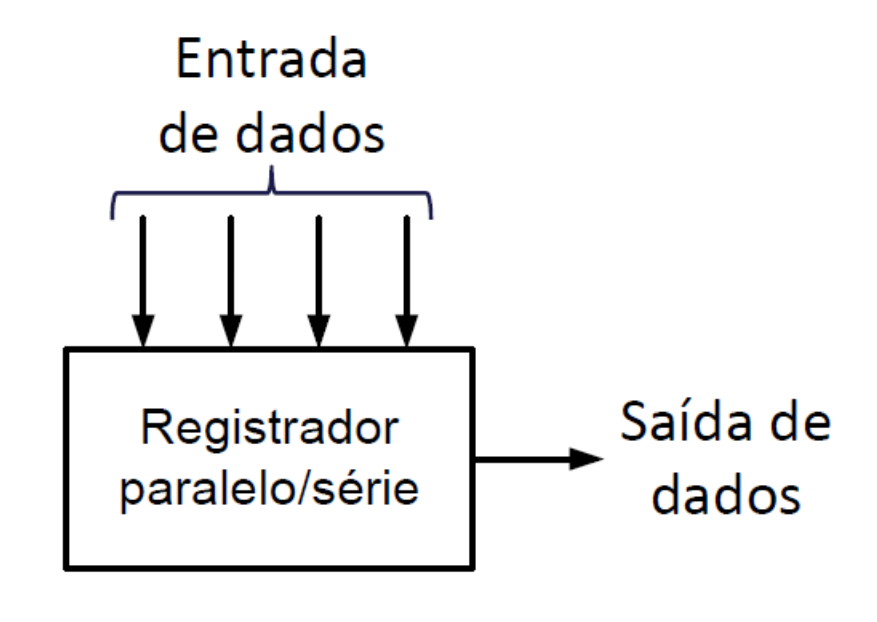
\includegraphics[width=0.65\textwidth]{figures/paralelo_serie.png}
\end{frame}

\begin{frame}{Paralelo-Paralelo}
\begin{itemize}
    \item Entrada e saída de todos os bits simultaneamente.
    \item Alta velocidade de operação.
\end{itemize}
\end{frame}

\begin{frame}{Exemplo - Paralelo-Paralelo}
\centering
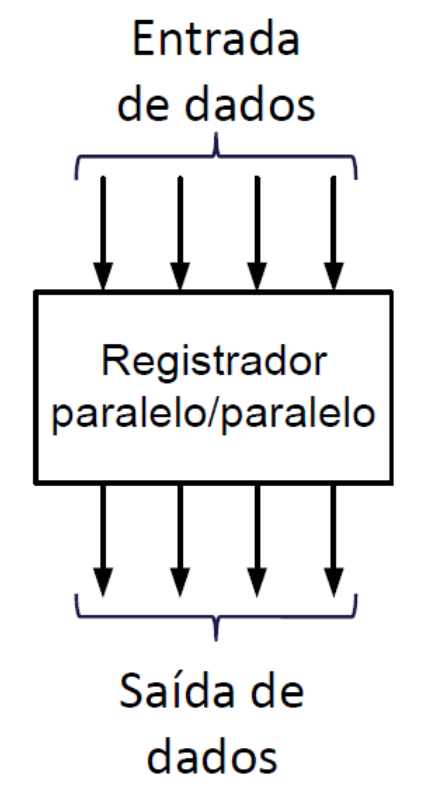
\includegraphics[width=0.3\textwidth]{figures/paralelo_paralelo.png}
\end{frame}


\begin{frame}{Registradores}
\begin{itemize}
    \item O valor lógico que está atualmente presente em A é transferido para o FF B na transição negativa (descida) do pulso transfer. Portanto, após esta transição, a saída B terá o mesmo valor de A.

 \item O grupo de FF é organizado de modo que os números binários a serem armazenados sejam deslocados de um FF para o FF seguinte, a cada pulso de clock. 
 \\
 
\centering
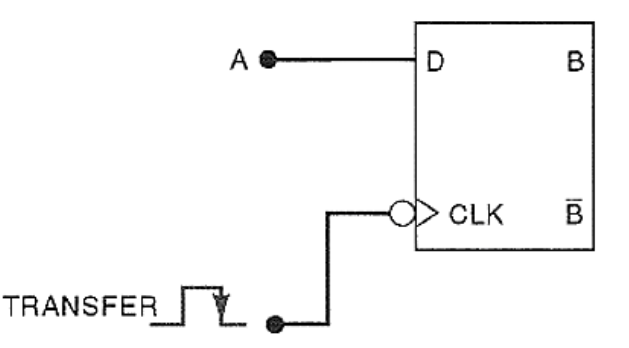
\includegraphics[width=0.4\textwidth]{figures/D_REGISTRADOR.png}

\end{itemize}
\end{frame}

\section{ Transferência Dados - Registrador 
}

\begin{frame}{Transferência Dados - Registrador }
\begin{itemize}
    \item Consiste em inserir dados na entrada do registrador, respeitando o número de bits, e efetuar o número de pulsos de clock necessários para que todo o dado seja inserido no registrador. 

\item O valor da saída X3 é transferido para X2, o de X2 para X1 e o de X1 para X0.

\item Quando ocorrer uma transição (disparo na borda de descida), cada FF assumirá o valor armazenado anteriormente pelo FF que está à sua esquerda.\\
 
\centering
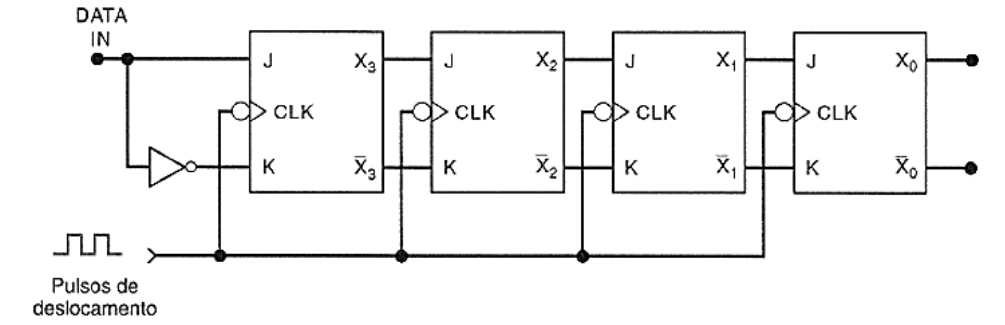
\includegraphics[width=0.7\textwidth]{figures/Tranf_dados.png}

\end{itemize}
\end{frame}



\begin{frame}{Transferência Dados - Registrador }
\begin{itemize}
    \item Exemplo: 
Possuindo o dado $110_{2}$, escreva a tabela verdade da transferência de dados para o registrador da figura abaixo, considerando que inicialmente ele foi limpo.\\
 
\centering
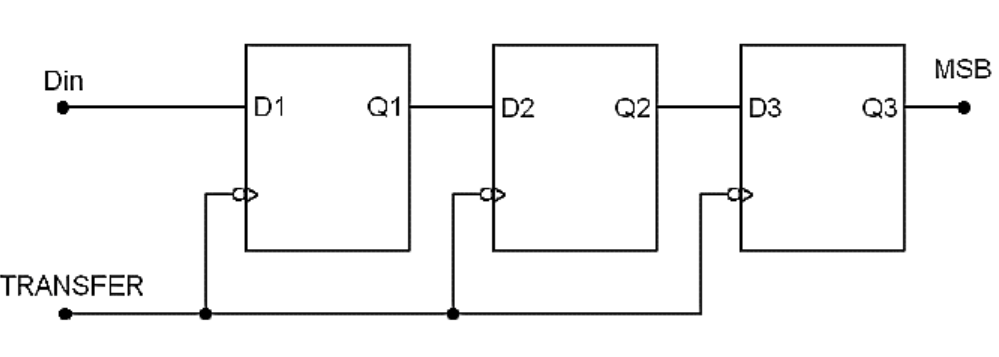
\includegraphics[width=0.7\textwidth]{figures/transf_d3bits.png}

\end{itemize}
\end{frame}


\begin{frame}{Transferência Dados - Registrador }
 
\centering
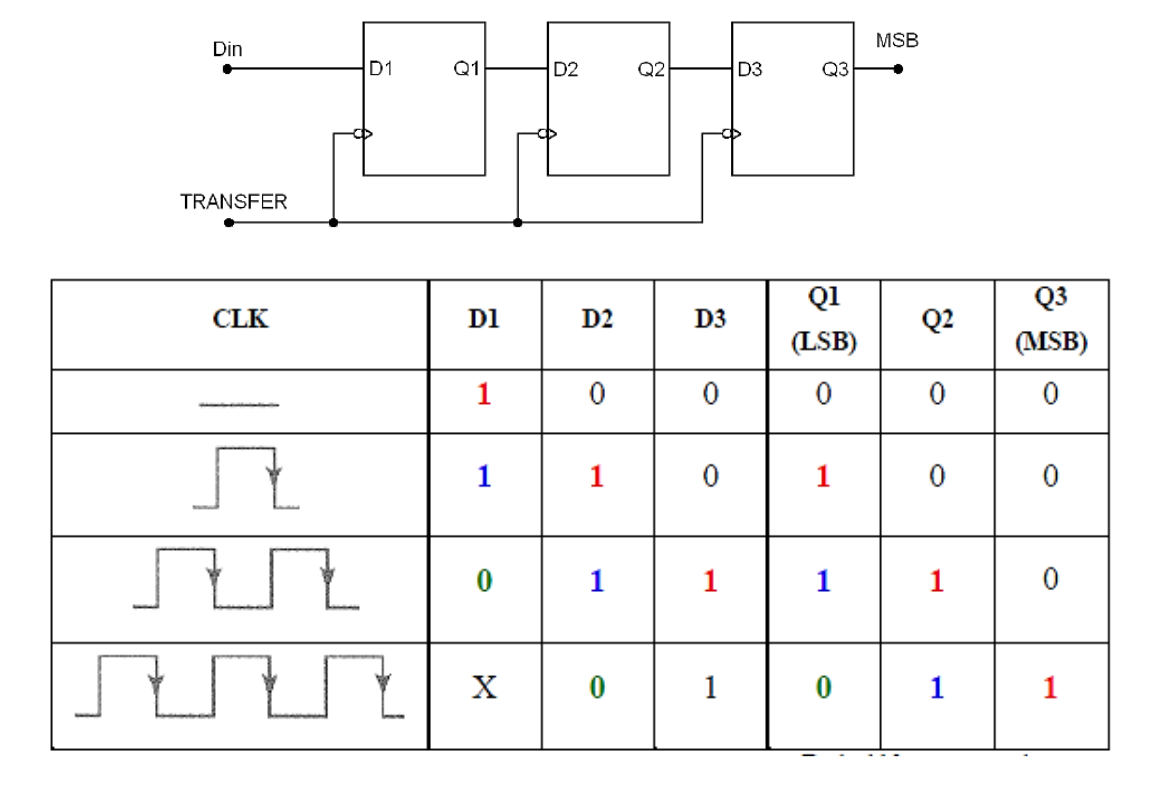
\includegraphics[width=0.7\textwidth]{figures/tabela_deslocador_ff_d.png}

\end{frame}


\begin{frame}{Transferência Dados - Registrador }
\begin{itemize}
    \item Dois registradores de deslocamento de três bits conectados de tal modo que o conteúdo do registrador X seja transferido serialmente (deslocado) para o registrador Y. 

\item Portanto, quando os pulsos de deslocamento são aplicados, a transferência de informação ocorre da seguinte forma: X2-> X1-> X0 -> Y2 -> Y1 -> Y0. 

\end{itemize}
 
\centering
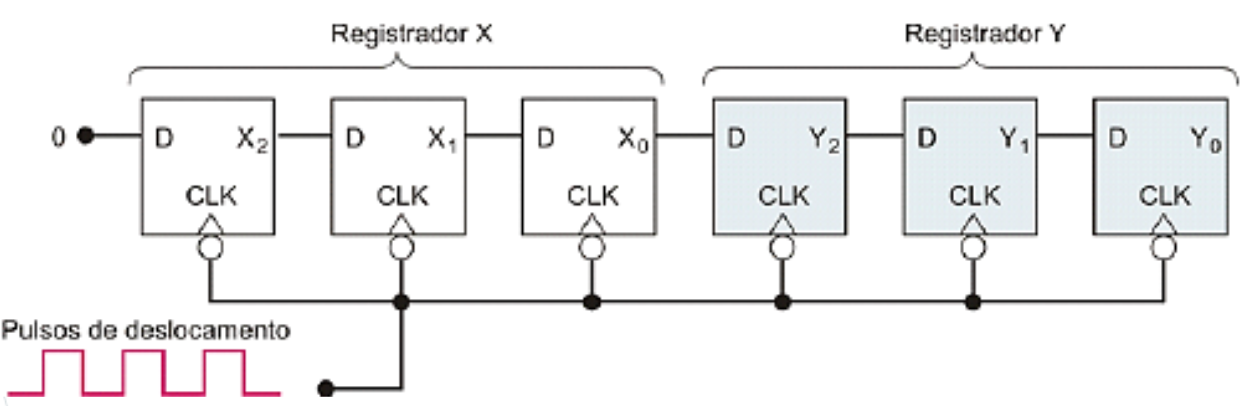
\includegraphics[width=0.7\textwidth]{figures/des_3valores.png}

\end{frame}


\begin{frame}{Transferência Dados - Registrador }
\begin{itemize}
    \item Supondo que inicialmente temos o dado $101_{2}$ armazenado no registrador X e que o registrador Y foi limpo, temos a seguinte tabela verdade abaixo: 

\end{itemize}
 
\centering
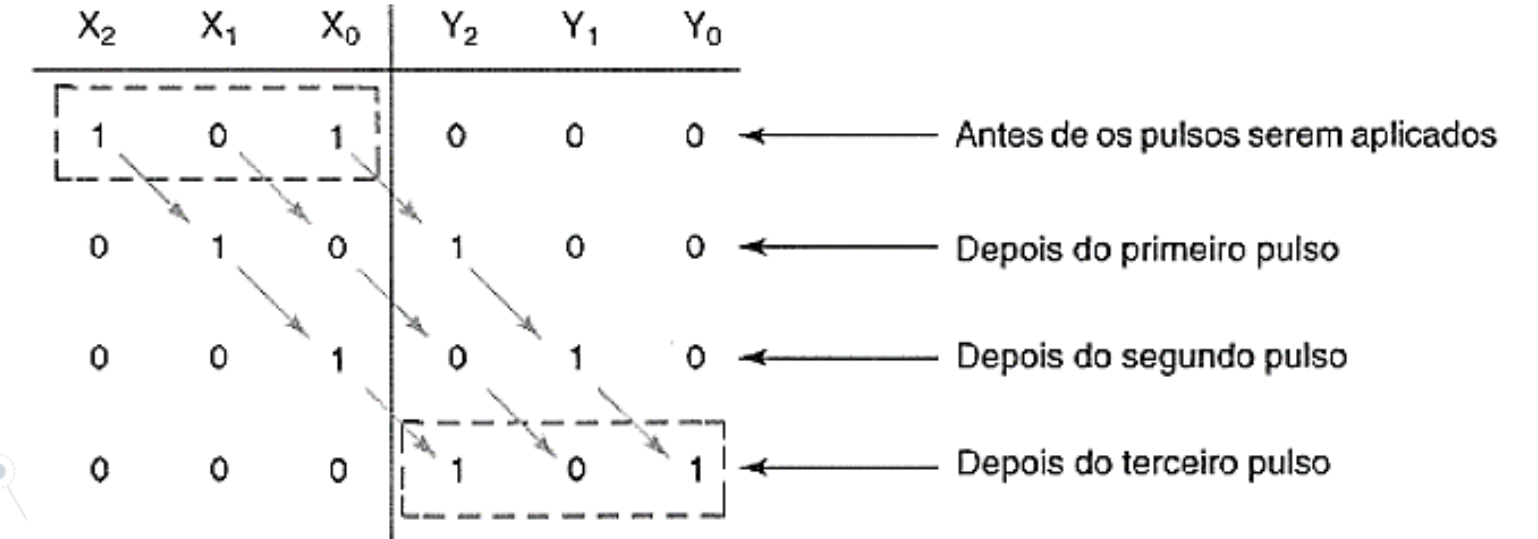
\includegraphics[width=0.8\textwidth]{figures/seq_clock.png}

\end{frame}


\begin{frame}{Transferência Dados - Registrador }
A partir dessa tabela podemos concluir que:
\begin{itemize}
    \item A cada descida do pulso de clock, cada FF assume o valor que foi armazenado no FF à sua esquerda, antes da ocorrência do pulso. 

    \item Após 3 pulsos, todo o conteúdo presente no registrador X está presente no registrador Y.

    \item Portanto, a transferência completa de 3 bits necessita de 3 pulsos de deslocamento. 


\end{itemize}


\end{frame}


\begin{frame}{Exemplo: Com o registrador série/série leve o bit 1 até a saída de dados
 }

\begin{figure}
\centering
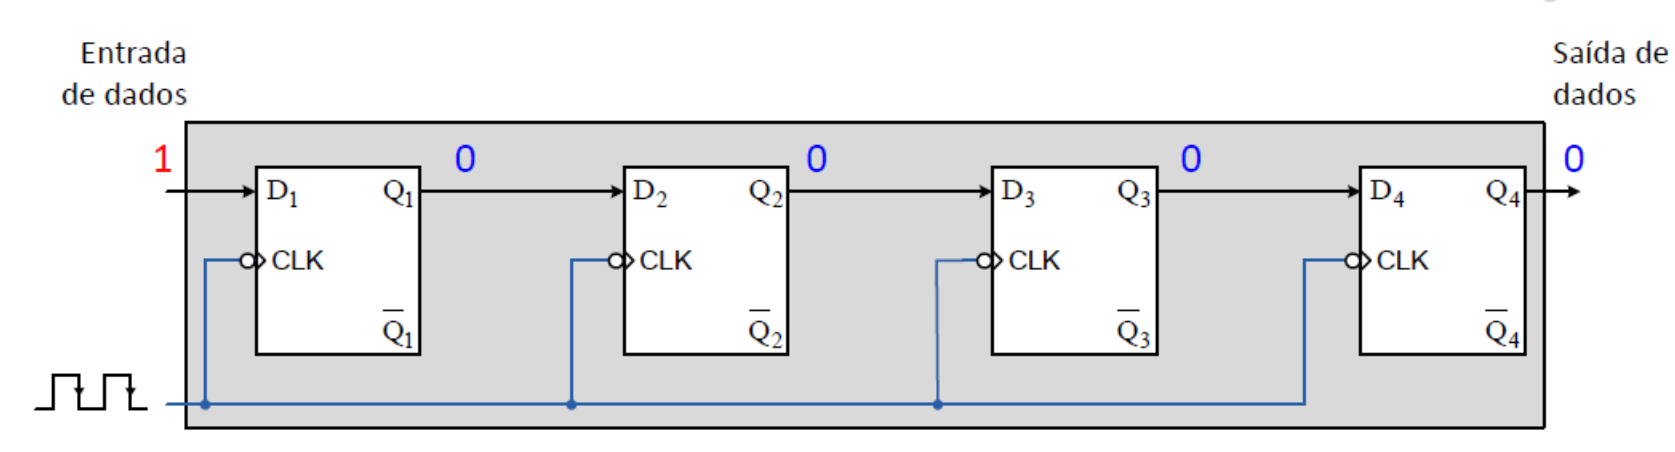
\includegraphics[width=0.9\textwidth]{figures/seq_1.png}
\end{figure}


\end{frame}


\begin{frame}{Exemplo: Com o registrador série/série leve o bit 1 até a saída de dados
 }

\begin{figure}
\centering
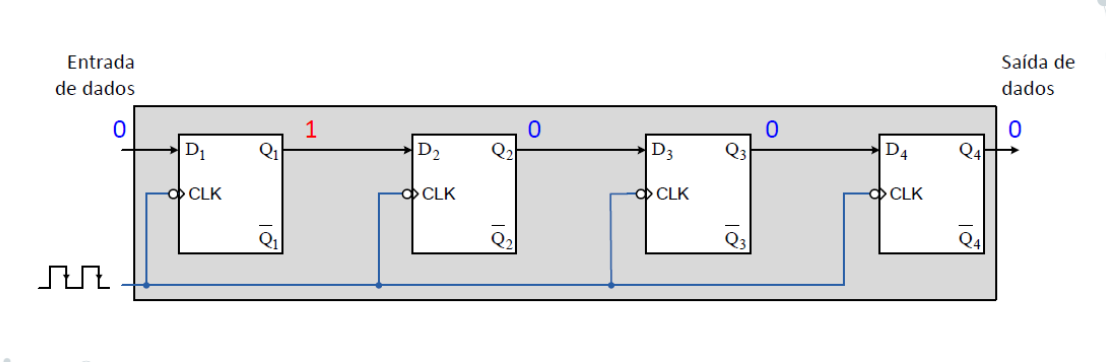
\includegraphics[width=0.9\textwidth]{figures/seq_2.png}
\end{figure}


\end{frame}

\begin{frame}{Exemplo: Com o registrador série/série leve o bit 1 até a saída de dados
 }

\begin{figure}
\centering
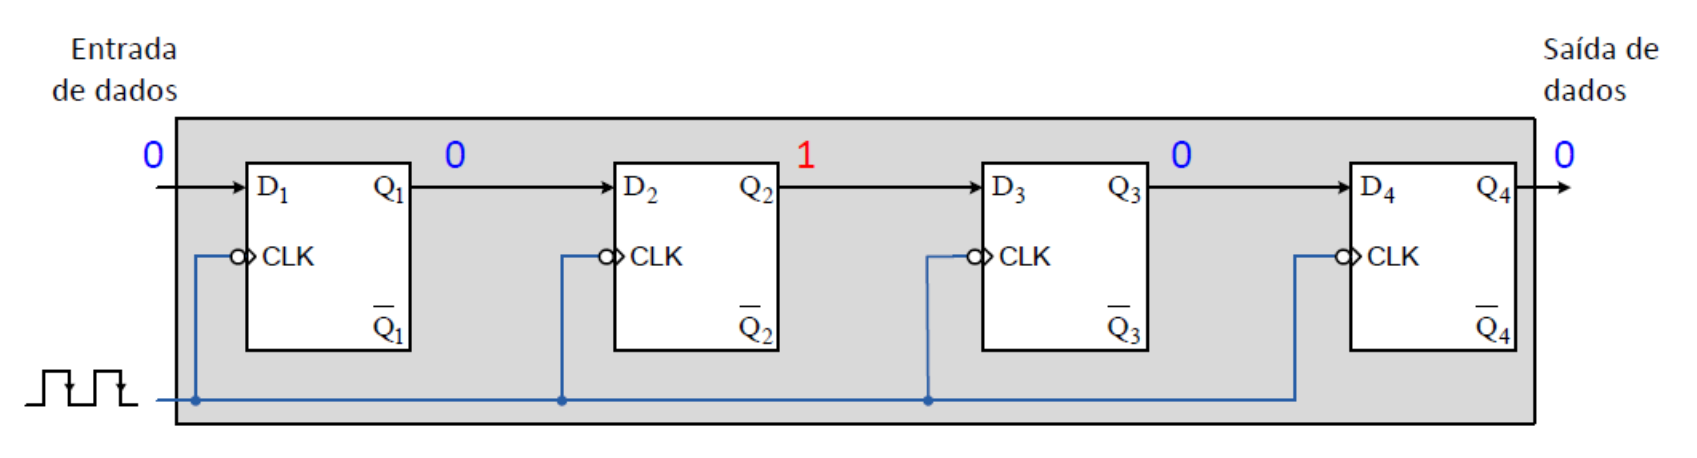
\includegraphics[width=0.9\textwidth]{figures/seq_3.png}
\end{figure}


\end{frame}

\begin{frame}{Exemplo: Com o registrador série/série leve o bit 1 até a saída de dados
 }

\begin{figure}
\centering
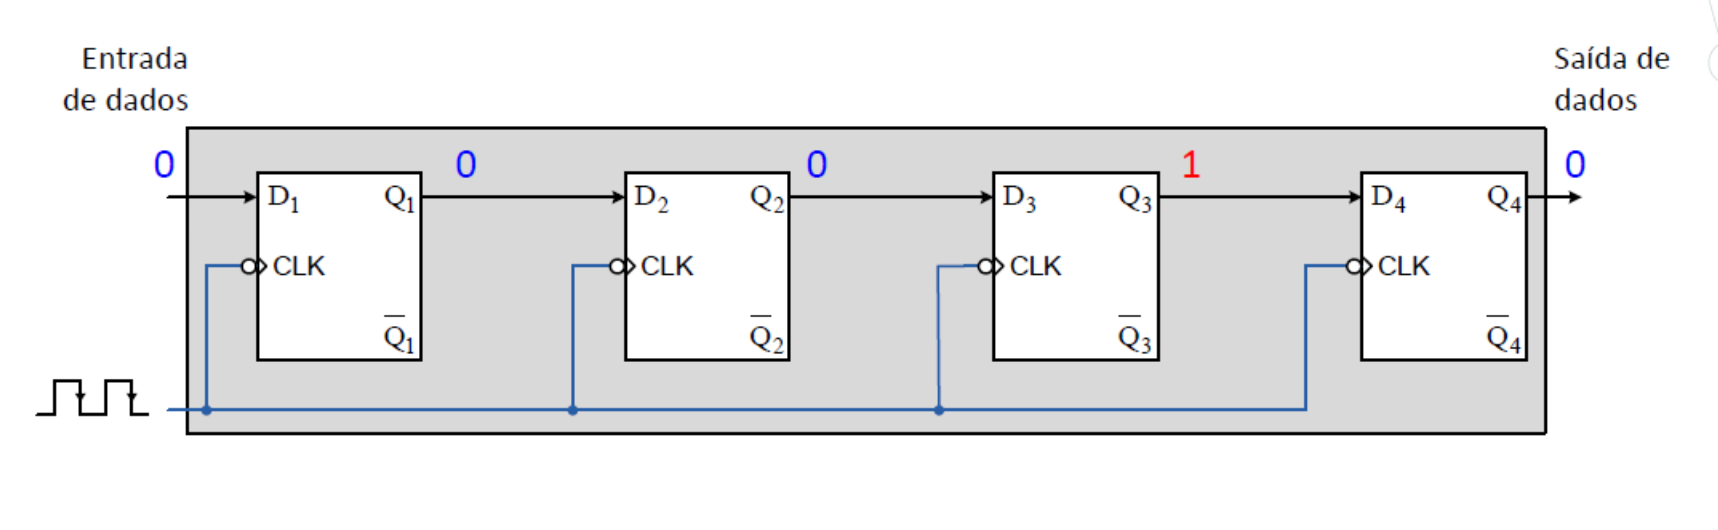
\includegraphics[width=0.9\textwidth]{figures/seq_4.png}
\end{figure}


\end{frame}



\begin{frame}{Exemplo: Com o registrador série/série leve o bit 1 até a saída de dados
 }

\begin{figure}
\centering
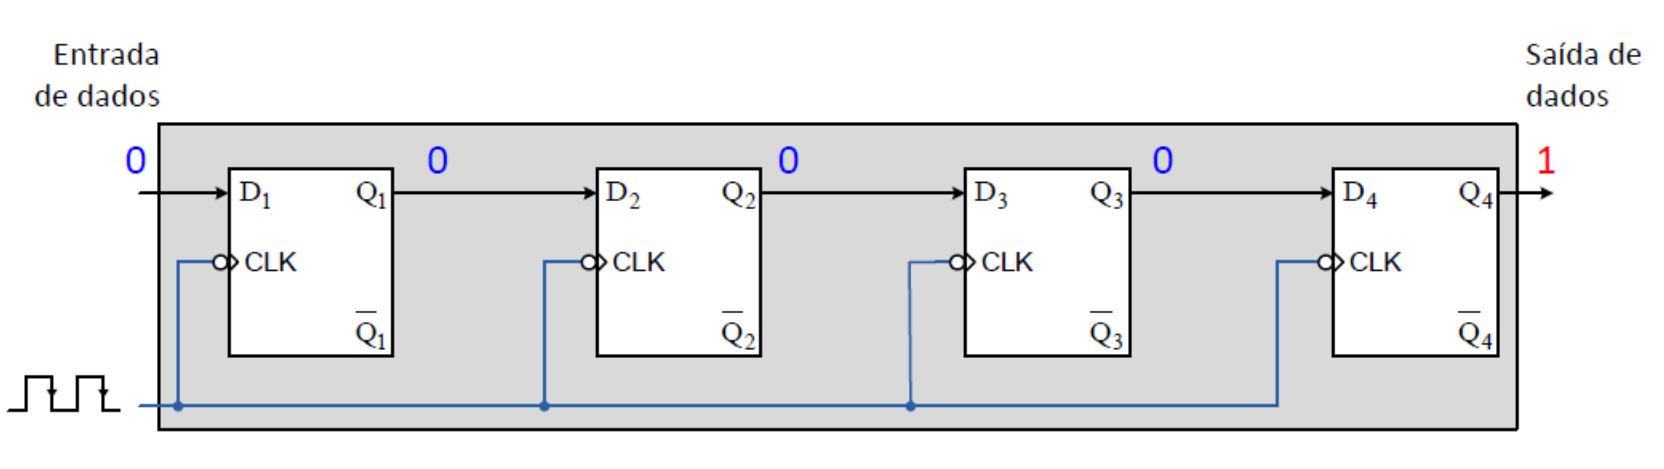
\includegraphics[width=0.9\textwidth]{figures/seq_5.png}
\end{figure}


\end{frame}


\begin{frame}{Transferência Paralela de Dados }

\begin{itemize}
\item O grupo de FF é organizado de maneira que o dado binário a ser armazenado seja transferido simultaneamente para todos os FF, com a aplicação de apenas 1 pulso de transferência ou clock. 

\item Consiste em inserir o dado a ser armazenado diretamente na entrada do registrador, efetuando-se 1 pulso de transferência.


\end{itemize}




\end{frame}



\begin{frame}{Transferência Paralela de Dados
 }

\begin{figure}
\centering
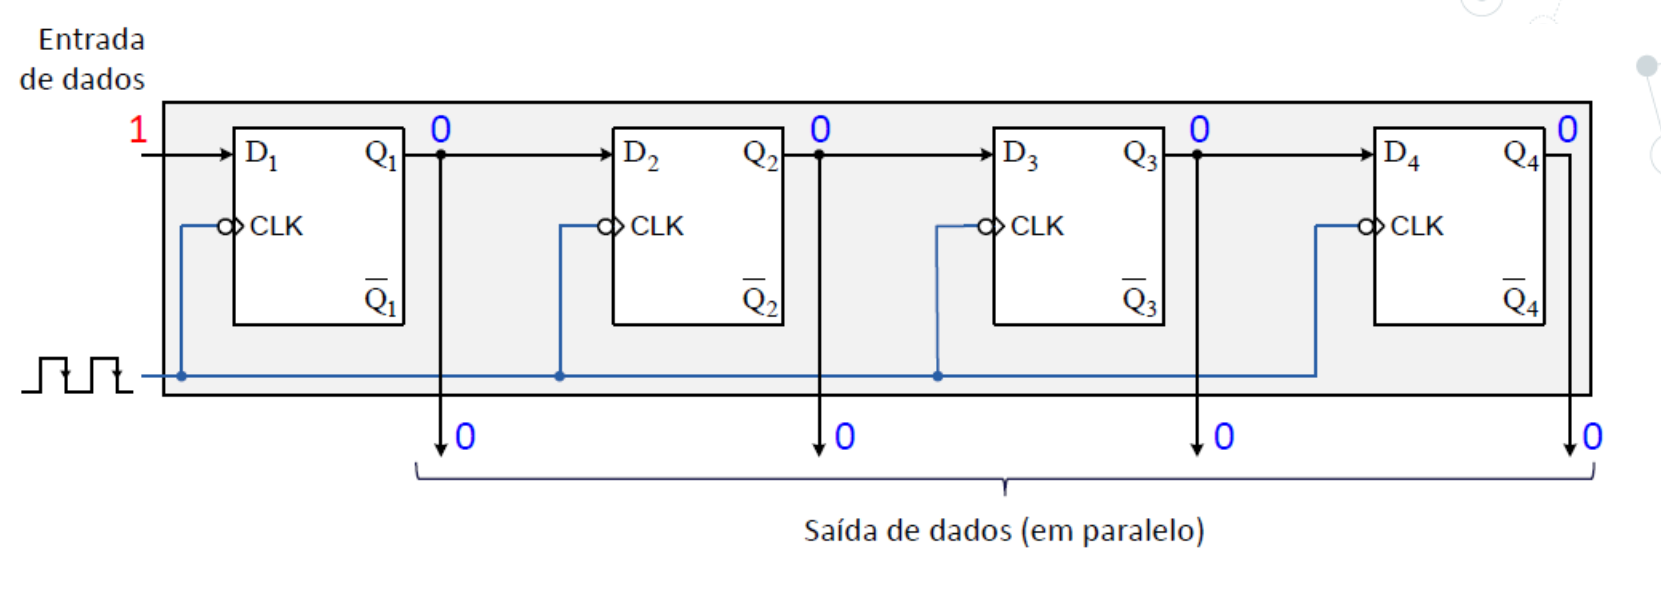
\includegraphics[width=0.9\textwidth]{figures/par_1.png}
\end{figure}


\end{frame}



\begin{frame}{Transferência Paralela de Dados
 }

\begin{figure}
\centering
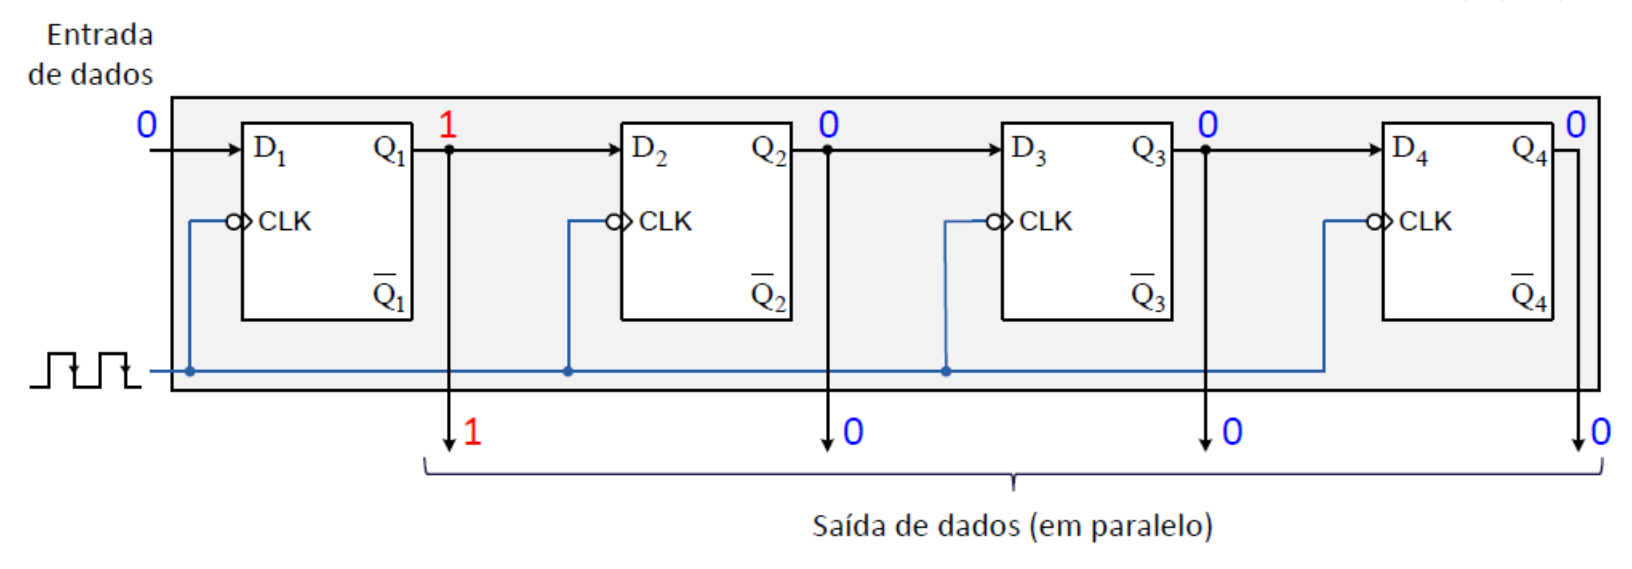
\includegraphics[width=0.9\textwidth]{figures/par_2.png}
\end{figure}


\end{frame}


\begin{frame}{Transferência Paralela de Dados
 }

\begin{figure}
\centering
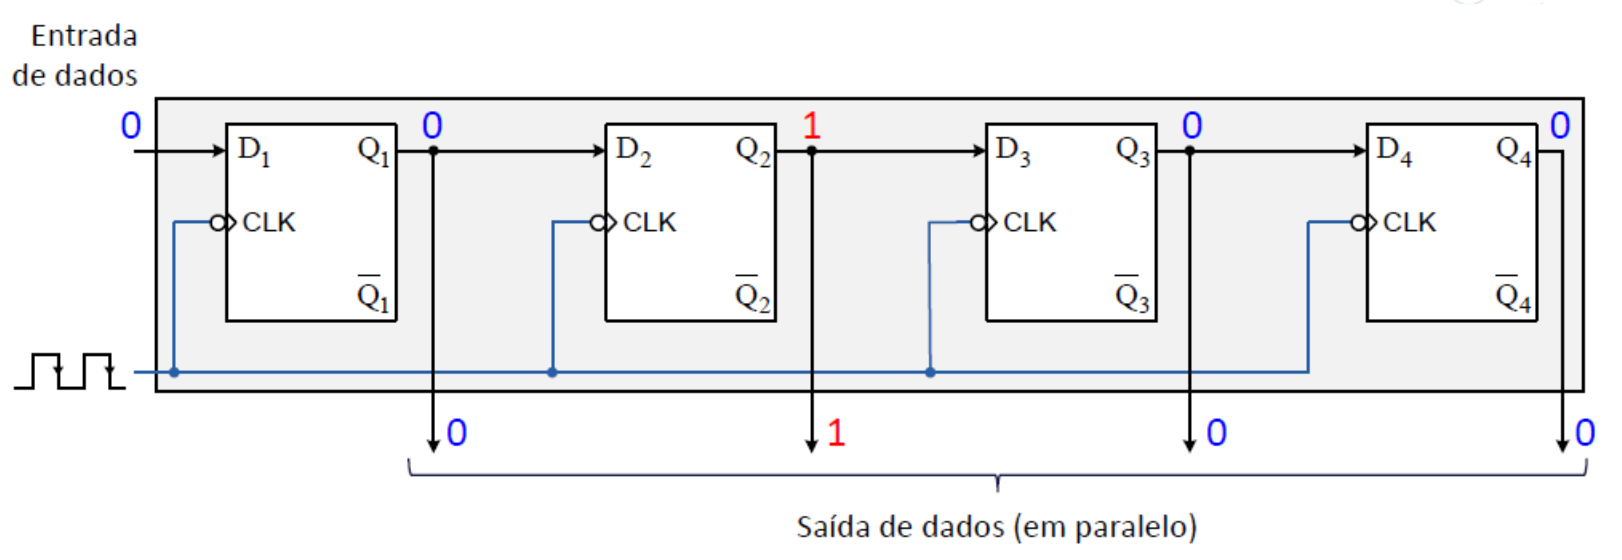
\includegraphics[width=0.9\textwidth]{figures/par_3.png}
\end{figure}


\end{frame}


\begin{frame}{Transferência Paralela de Dados
 }

\begin{figure}
\centering
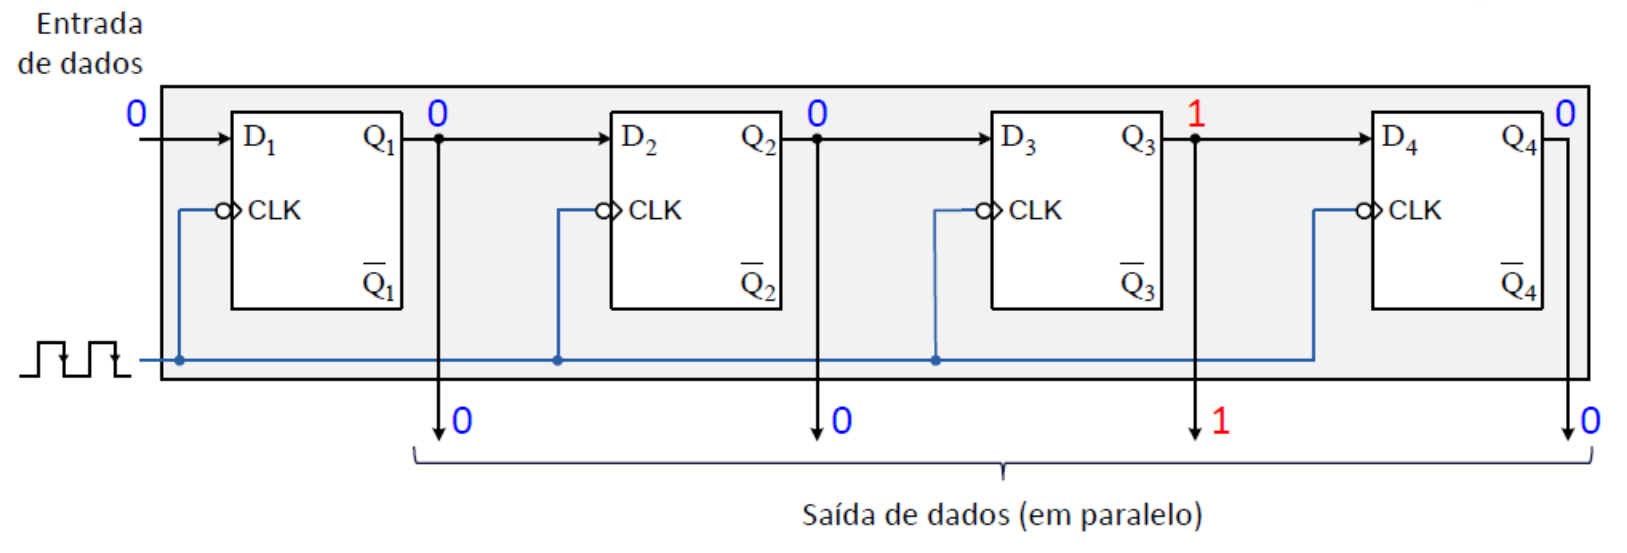
\includegraphics[width=0.9\textwidth]{figures/par_4.png}
\end{figure}


\end{frame}


\begin{frame}{Transferência Paralela de Dados
 }

\begin{figure}
\centering
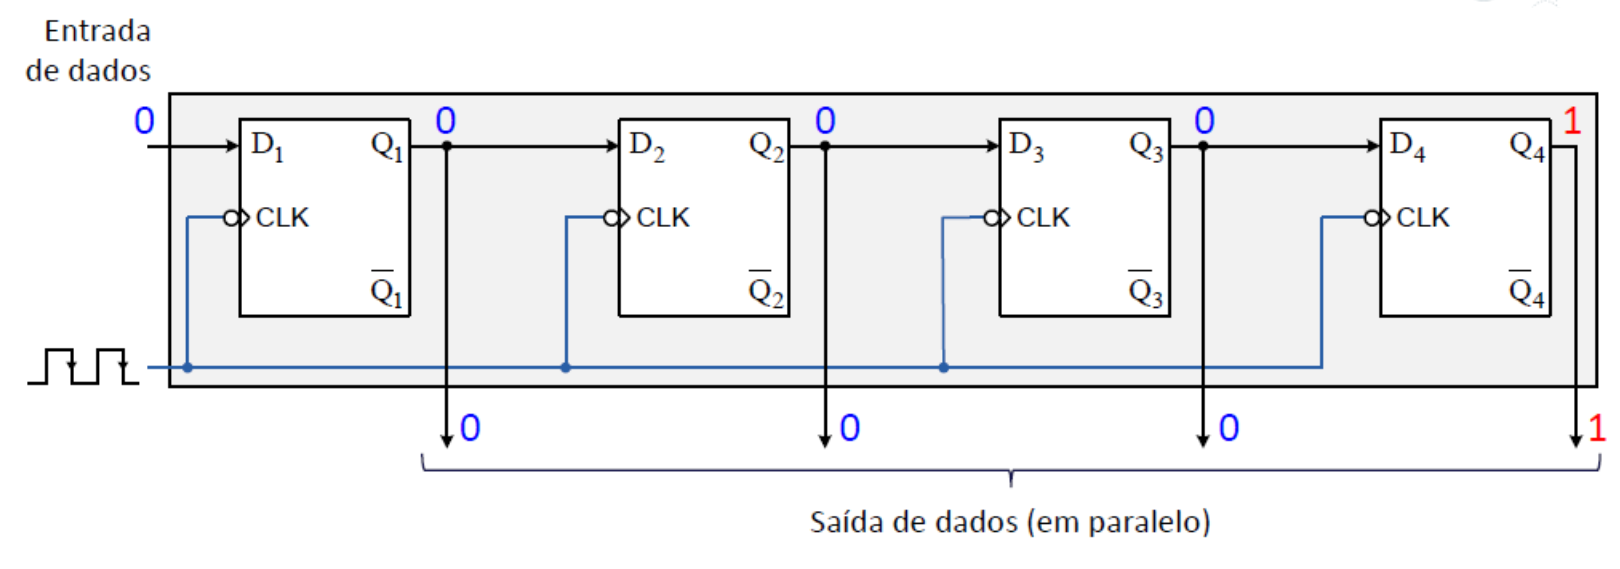
\includegraphics[width=0.9\textwidth]{figures/par_5.png}
\end{figure}


\end{frame}


\begin{frame}{Transferência Paralela de Dados
 }

\begin{itemize}
 \item Dois registradores, X e Y, interligados para executar uma transferência paralela de dados, ou seja, após a aplicação de 1 pulso de transferência, temos todo o conteúdo de X armazenado também em Y. 

\item A transferência paralela de dados entre registradores não altera o conteúdo da fonte, enquanto na transferência serial altera o gradativamente o valor do registrador que atua como fonte de dados. 

\end{itemize}


\end{frame}

\begin{frame}{Transferência Paralela de Dados
 }

\begin{figure}
\centering
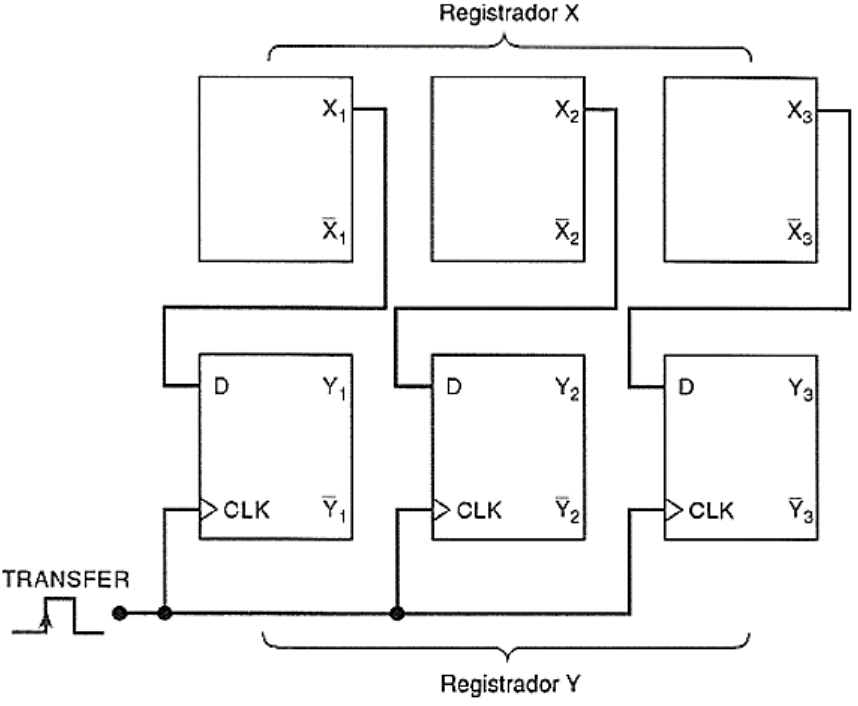
\includegraphics[width=0.7\textwidth]{figures/paralelo.png}
\end{figure}


\end{frame}

\begin{frame}{Serial x Paralela
 }

\begin{figure}
\centering
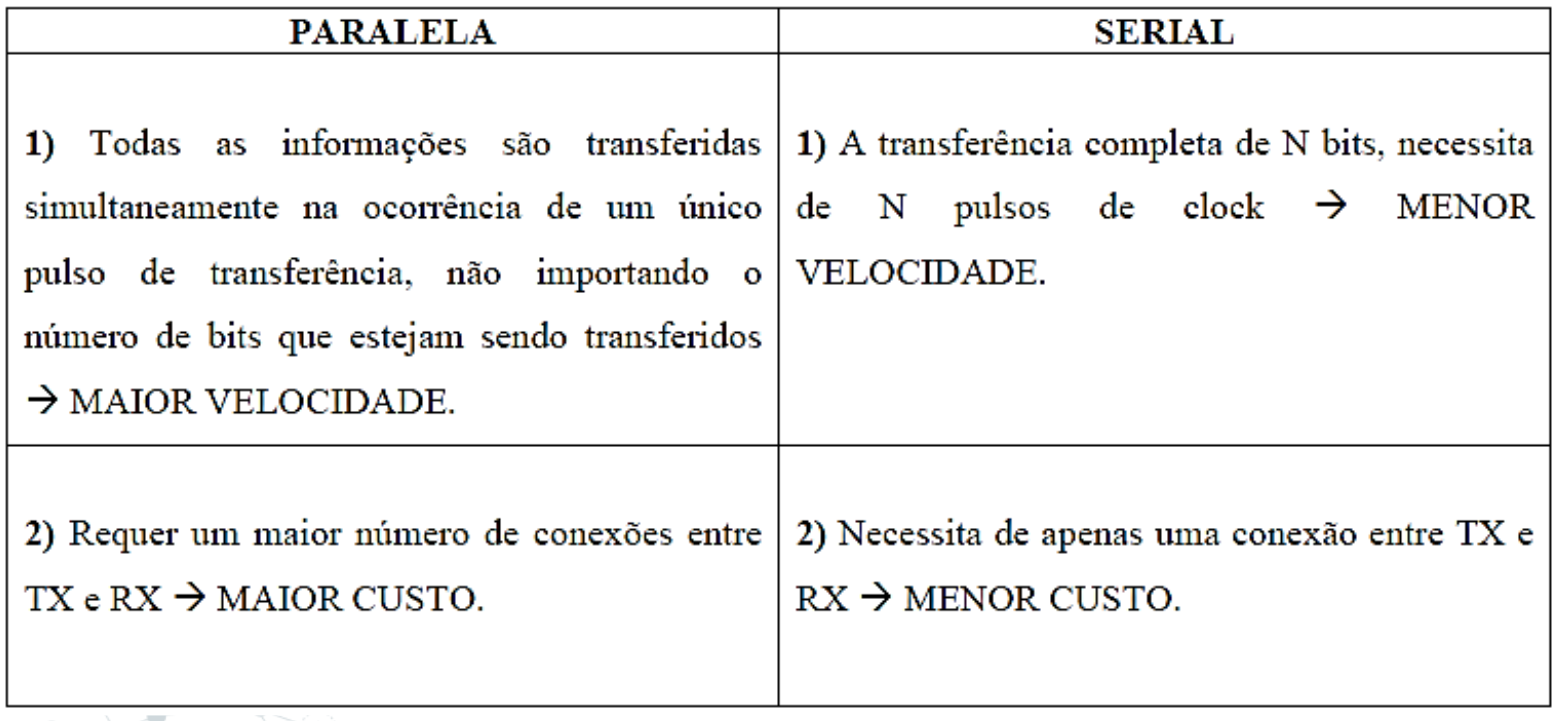
\includegraphics[width=0.9\textwidth]{figures/serial_paralela.png}
\end{figure}


\end{frame}


\section{Aplicações e Conclusão}

\begin{frame}{Aplicações}
\begin{itemize}
    \item Armazenamento temporário de dados.
    \item Conversão de dados entre dispositivos.
    \item Contadores, somadores e multiplicadores.
\end{itemize}
\end{frame}

\begin{frame}{Conclusão}
\begin{figure}
\centering
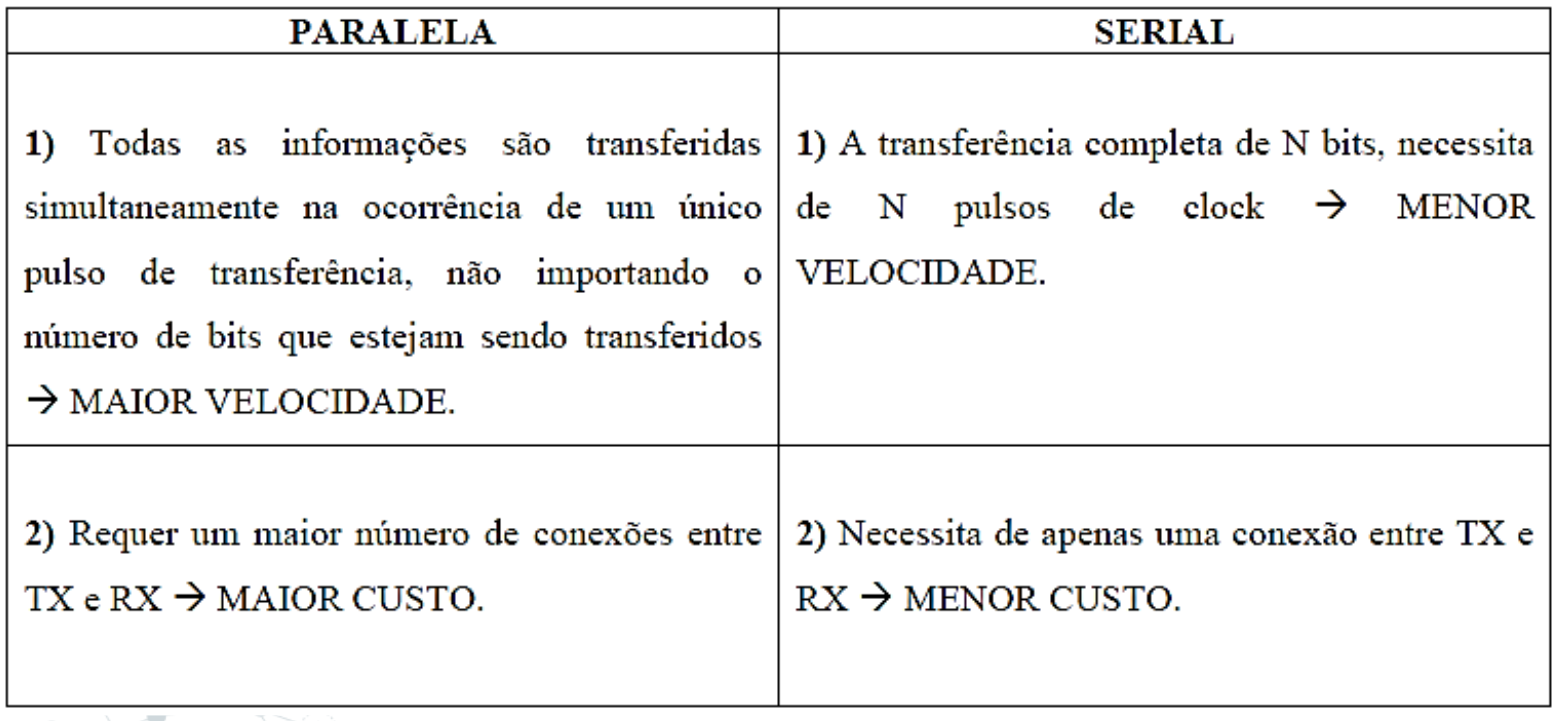
\includegraphics[width=0.9\textwidth]{figures/serial_paralela.png}
\end{figure}
\end{frame}


\section{Exercício}

\begin{frame}{Exercício}
\begin{figure}
\centering
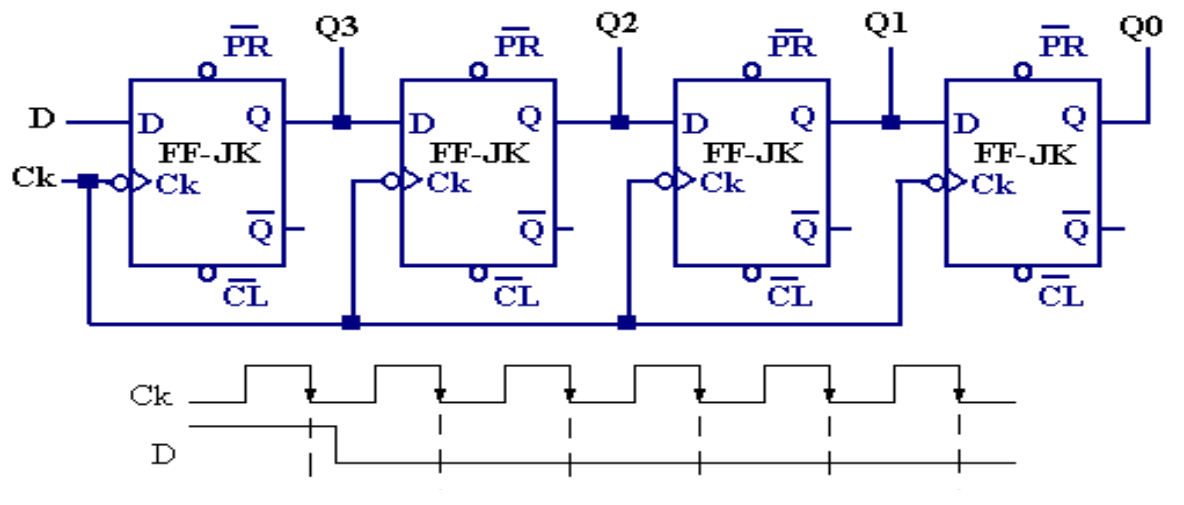
\includegraphics[width=0.9\textwidth]{figures/exer.png}
\end{figure}
\end{frame}


\section{Referências}

\begin{frame}{Referências}
\begin{enumerate}
    \item HARRIS, D. M.; HARRIS, S. L. Digital Design and Computer Architecture. Elsevier, 2015.
    \item GROUT, I. Digital Systems Design with FPGAs and CPLDs. Elsevier, 2008.
    \item SILVINA HANONO WACHMAN. MIT 6.004 - Sequential Circuits. YouTube, 2024.
\end{enumerate}
\end{frame}

\end{document}